\documentclass[border=3pt,tikz]{standalone}
% Shared look for every TikZ figure in these notes.
% Included by each standalone figure file; also keeps the figures consistent
% with the colours used in the PDF and on the website.

\usepackage{tikz}
\usepackage{pgfplots}
\pgfplotsset{compat=1.18}
\usetikzlibrary{arrows.meta, decorations.markings, decorations.pathmorphing,
                patterns, calc, positioning}
\usepackage{amsmath}

% Series colours are the three validated categorical slots also used by the
% interactive widgets, so a path drawn in the printed notes and the same path on
% the website are the same colour. They clear the colour-vision-deficiency and
% contrast checks as a set; every path is direct-labelled as well, so colour is
% never the only thing carrying identity.
\definecolor{duPurple}{HTML}{68246D}
\definecolor{duBlue}{HTML}{2A78D6}
\definecolor{duRed}{HTML}{EB6834}
\definecolor{duGreen}{HTML}{1BAF7A}
\definecolor{duGrey}{HTML}{4D4D4D}

\tikzset{
  % heavier default lines and arrow tips, so diagrams stay clear when zoomed
  every picture/.append style = {line width=0.7pt, >={Stealth[length=3mm]}},
  axisline/.style   = {-{Stealth[length=3.4mm]}, line width=1.0pt, black},
  path1/.style      = {duBlue,   line width=1.6pt},
  path2/.style      = {duRed,    line width=1.6pt},
  path3/.style      = {duGreen,  line width=1.6pt},
  statedot/.style   = {circle, fill=black, inner sep=1.8pt},
  arrowhead/.style  = {decoration={markings,
                        mark=at position #1 with {\arrow{Stealth[length=3.4mm]}}},
                       postaction={decorate}},
  lbl/.style        = {font=\normalsize},
  slbl/.style       = {font=\small, duGrey},
  workfill/.style   = {duPurple, opacity=0.16},
}

% larger labels in plots as well
\pgfplotsset{every axis/.append style={label style={font=\normalsize}, tick label style={font=\small}, line width=0.9pt}}

% Steady flow through a control volume: a fluid element enters at the bottom
% left and another leaves at the top right; the CV (dashed) stays the same.
\begin{document}
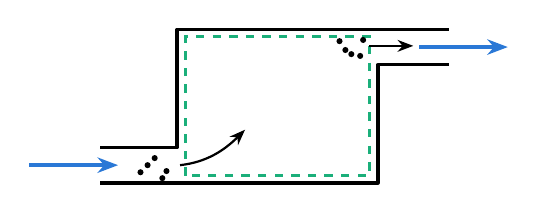
\begin{tikzpicture}[x=0.75cm, y=0.75cm,
    wall/.style={line width=1.2pt, line join=round},
    flow/.style={-{Stealth[length=2.6mm]}, duBlue, line width=1.3pt},
    move/.style={-{Stealth[length=2mm]}, line width=0.8pt}]
  % duct: inlet bottom left, box, exit top right
  \draw[wall] (-1.3,0.6) -- (0,0.6) -- (0,2.6) -- (4.6,2.6);
  \draw[wall] (4.6,2.0) -- (3.4,2.0) -- (3.4,0) -- (-1.3,0);
  % control volume
  \draw[duGreen, dashed, line width=1.1pt] (0.15,0.12) rectangle (3.25,2.48);
  % fluid element entering, and one leaving
  \foreach \p in {(-0.62,0.18),(-0.38,0.42),(-0.18,0.2),(-0.5,0.3),(-0.25,0.08)}
    \fill \p circle (1.1pt);
  \draw[move] (0.05,0.3) .. controls (0.5,0.35) and (0.8,0.55) .. (1.15,0.9);
  \foreach \p in {(2.75,2.4),(2.95,2.18),(3.15,2.42),(2.85,2.25),(3.1,2.15)}
    \fill \p circle (1.1pt);
  \draw[move] (3.25,2.32) -- (4.0,2.32);
  % flow in and out
  \draw[flow] (-2.5,0.3) -- (-1.0,0.3);
  \draw[flow] (4.1,2.3) -- (5.6,2.3);
\end{tikzpicture}
\end{document}
